% Evidence-gated benchmark framework (replaces the separate hub and architecture drawings).
% Drawn at IEEE double-column width (7.16 in); include at \textwidth without scaling.
% Model borders use the same colors as the data figures (M1 sky blue, M2 orange, M3 green).
% Build: pdflatex fig_evidence_gated_framework.tex
\documentclass[10pt,border=1pt]{standalone}
\usepackage[helvet]{sfmath}
\usepackage[scaled=1.0]{helvet}
\renewcommand{\familydefault}{\sfdefault}
\usepackage{tikz}
\usetikzlibrary{arrows.meta,positioning,shapes.geometric,calc}

\definecolor{mone}{HTML}{56B4E9}
\definecolor{mtwo}{HTML}{E69F00}
\definecolor{mthree}{HTML}{009E73}
\definecolor{ink}{HTML}{1A1A1A}
\definecolor{verify}{HTML}{DCEAF5}
\definecolor{diagnose}{HTML}{FBF3C4}

\begin{document}
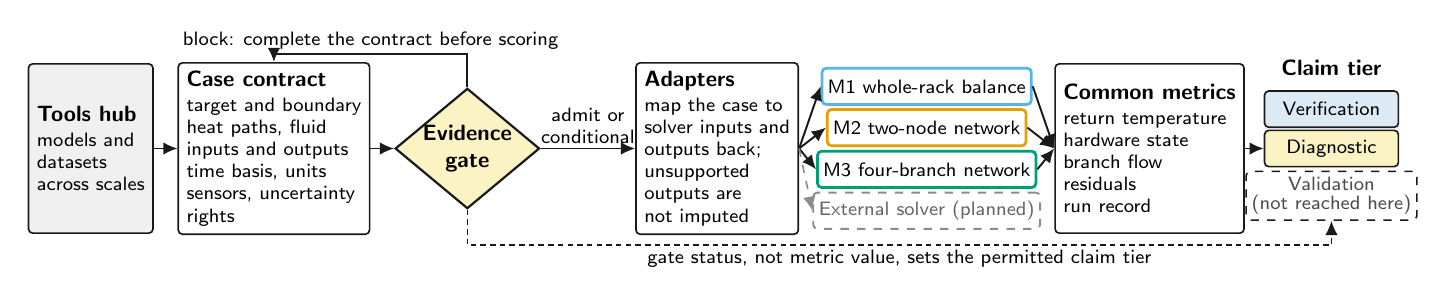
\begin{tikzpicture}[
    x=1cm, y=1cm,
    font=\scriptsize,
    >={Latex[length=1.8mm,width=1.6mm]},
    box/.style={draw=ink, line width=0.6pt, rounded corners=1.5pt, align=left, inner sep=3pt, minimum height=2.15cm},
    model/.style={draw, line width=1.0pt, rounded corners=1.5pt, minimum width=2.4cm, minimum height=0.46cm, align=center, fill=white, inner sep=2pt},
    tier/.style={draw=ink, line width=0.6pt, rounded corners=1.5pt, minimum width=1.7cm, minimum height=0.46cm, align=center, inner sep=2pt},
    flow/.style={->, line width=0.7pt, draw=ink},
  ]
  % ------------------------------------------------------------------ boxes
  \node[box, fill=black!6] (hub) at (0,0)
    {{\footnotesize\bfseries Tools hub}\\[1pt] models and\\ datasets\\ across scales};
  \node[box, right=0.3cm of hub] (contract)
    {{\footnotesize\bfseries Case contract}\\[1pt] target and boundary\\ heat paths, fluid\\ inputs and outputs\\ time basis, units\\ sensors, uncertainty\\ rights};
  \node[diamond, draw=ink, line width=0.8pt, fill=diagnose, aspect=1.2, inner sep=0pt, align=center, font=\footnotesize\bfseries, right=0.3cm of contract] (gate) {Evidence\\gate};
  \node[box, right=1.2cm of gate] (adapters)
    {{\footnotesize\bfseries Adapters}\\[1pt] map the case to\\ solver inputs and\\ outputs back;\\ unsupported\\ outputs are\\ not imputed};
  \coordinate (mc) at ($(adapters.east)+(1.62,0)$);
  \node[model, draw=mone]   (m1) at ($(mc)+(0,0.79)$)  {M1 whole-rack balance};
  \node[model, draw=mtwo]   (m2) at ($(mc)+(0,0.265)$) {M2 two-node network};
  \node[model, draw=mthree] (m3) at ($(mc)+(0,-0.265)$) {M3 four-branch network};
  \node[model, draw=black!45, dashed, text=black!60, line width=0.7pt] (mx) at ($(mc)+(0,-0.79)$) {External solver (planned)};
  \node[box, anchor=west] (metrics) at ($(mc)+(1.62,0)$)
    {{\footnotesize\bfseries Common metrics}\\[1pt] return temperature\\ hardware state\\ branch flow\\ residuals\\ run record};
  \coordinate (tc) at ($(metrics.east)+(1.1,0)$);
  \node[font=\footnotesize\bfseries] (tiertitle) at ($(tc)+(0,1.03)$) {Claim tier};
  \node[tier, fill=verify]   (verification) at ($(tc)+(0,0.5)$)  {Verification};
  \node[tier, fill=diagnose] (diagnostic)   at (tc)    {Diagnostic};
  \node[tier, dashed, fill=white, text=black!70] (validation) at ($(tc)+(0,-0.6)$) {Validation\\[-1pt](not reached here)};

  % ------------------------------------------------------------------ main flow
  \draw[flow] (hub.east) -- (contract.west);
  \draw[flow] (contract.east) -- (gate.west);
  \draw[flow] (gate.east) -- node[above, align=center, inner sep=1.5pt] {admit or\\conditional} (adapters.west);
  \foreach \m in {m1, m2, m3} {
    \draw[flow] (adapters.east) -- (\m.west);
    \draw[flow] (\m.east) -- (metrics.west);
  }
  \draw[->, line width=0.6pt, draw=black!45, dashed] (adapters.east) -- (mx.west);
  \draw[flow] (metrics.east) -- (diagnostic.west);

  % ------------------------------------------------------------------ block loop
  \draw[flow] (gate.north) -- ++(0,0.42) -| node[pos=0.25, above, inner sep=1.5pt] {block: complete the contract before scoring} (contract.north);

  % ------------------------------------------------------------------ gate status caps the claim
  \draw[->, line width=0.6pt, draw=ink, dash pattern=on 2pt off 1.5pt] (gate.south) -- ++(0,-0.45) -| node[pos=0.25, below, inner sep=1.5pt] {gate status, not metric value, sets the permitted claim tier} (validation.south);
\end{tikzpicture}
\end{document}
